\chapter{Desenvolvimento do modelo OLAP}

descrever como foi feito o levantamento dos residuos mais interesantes. Explicar que a lista dos mais presentes foi comparada com uma lista originalmente desenvolvida por um especialista de dominio. Encontrou se casos que estavam e nao estavam na lista, os que nao apareciam na lista constituem de residuos que se ficam ˜proximos”ao sitio de ligação, mas que na realidade estão fora do sítio.

descrever como  adicionar novas dimensoes baseadas em novos residuos

\section{Identificação de métricas}
Conforme visto no capítulo de referencial teórico, a FEB é um dos métodos utilizados para mensurar a qualidade de uma docagem molecular. Consequentemente a FEB se torna uma das métricas a ser levada em consideração para responder às questões de negócio elaboradas pelos especialistas de domínio. Outra métrica que será utilizada é o RMSD pois assim como a FEB ele também fornece uma forma de avaliar a qualidade da docagem. Estas duas métricas em conjunto dão uma visão para os especialistas de quão satisfatório foi o processo de docagem para uma determinada iteração.

A importância destas duas métricas para os especialistas se deve ao proposito distinto de cada uma delas. Enquanto a FEB mede a qualidade da docagem no aspecto termodinâmico da questão, o RMSD tem como natureza avaliar geometricamente como estão dispostas as moléculas do resíduo e ligante.

\section{Identificação dos resíduos relevantes}
Um dos pontos mais importantes para responder aos questionamentos dos especialistas de domínio e fundamental para composição das dimensões, era saber quais eram os resíduos mais relevantes. A enzima InhA possui 268 resíduos \cite{KARANADUNOSM09} e o processo de identificação dos mais importantes leva em consideração o número de contatos do resíduo com o ligante. Na base de informações que foi resultado do processo de simulação de docagem, cada resíduo é representado por uma tripla contendo a sua localização espacial nos eixos x, y e z.

De acordo com o especialista de domínio, para ser considerado contato do resíduo com o ligante é preciso estar em uma distância entre 2 e 4 angstrom. Valores inferiores a 2 angstrom são descartados por serem considerados uma sobreposição. Desta forma é utilizado o cálculo da distância euclidiana entre os átomos do resíduo e do ligante \cite{KARANADUNOSM09} para encontrar estes valores, desprezando os átomos de hidrogênio conforme determinação dos especialistas de domínio. Quanto maior o número de contatos do resíduo com o ligante, mais relevante para o especialista é o resíduo. As regras para elencar os resíduos mais relevantes podem ser sumarizadas da seguinte forma:

\begin{enumerate}
    \item Distância de 2 a 4 angstrom são considerados contatos.
    \item Distância inferior a 2 angstrom são desconsideradas. 
    \item Descarte do cálculo para os átomos de hidrogênio.
    \item Quanto mais contatos, mais relevante.
\end{enumerate}

Após execução dos algoritmos elaborados dentro do trabalho para coletar estas informações, foram identificados 15 resíduos mais relevantes que posteriormente foram avaliados pelos especialistas e reduzidos a uma lista de 10 resíduos. Com base em uma lista anteriormente elaborada por um especialista de domínio, conforme mostrado na figura 5.1, os 5 resíduos que sobraram dos 15 iniciais foram identificados como casos onde a proteína, devido a flexibilidade, abriu uma cavidade acima da cavidade do substrato, permitindo ligações do ligante fora da cavidade do substrato.

\begin{figure}[h]
        \center
        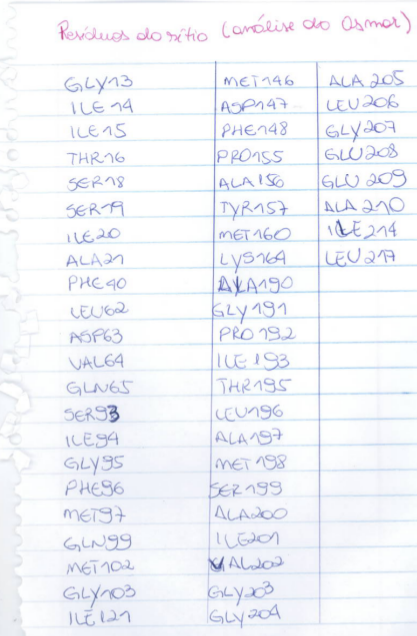
\includegraphics[width=12cm]{images/ListaProfOsmar.png}
        \label{fig:rddworkflow}
        \caption{Lista dos principais resíduos do Professor Osmar}
\end{figure}

A figura 5.2 mostra os 15 resíduos que foram identificados inicialmente. Aqueles indicados em vermelho são os considerados importantes e os indicados em branco foram descartados porque ficaram fora do sítio de ligação.

\begin{figure}[h]
        \center
        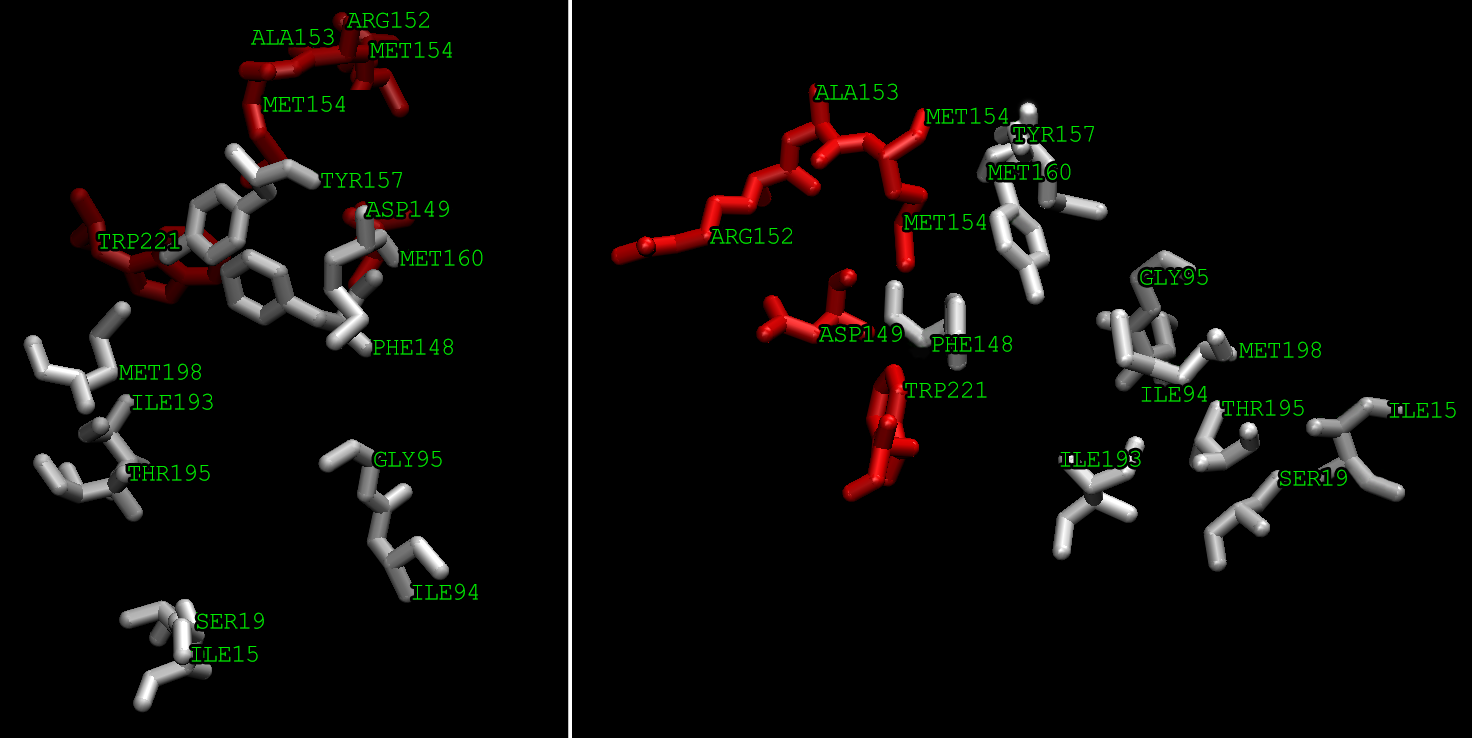
\includegraphics[width=10cm]{images/avaliacao_Residuos_nomes.png}
        \label{fig:rddworkflow}
        \caption{Lista inicial dos 15 resíduos mais relevantes}
\end{figure}

Com base nestas prerrogativas foram selecionados os 10 principais resíduos mais relevantes para responder às questões dos especialistas conforme mostrado.

\begin{itemize}
	\item PHE\_148 (Phenylalanine)
	\item ILE\_193 (Isoleucine)
	\item GLY\_95 (Glycine)
	\item THR\_195 (Threonine)
	\item ILE\_94 (Isoleucine)
	\item MET\_198 (Methionine)
	\item MET\_160 (Methionine)
	\item SER\_19 (Serine)
	\item ILE\_15 (Isoleucine)
	\item TYR\_157 (Tyrosine)
\end{itemize}



\section{Dimensões}
	mostrar hierarquias de dimensoes
	
\section{Construção do modelo no Analisys Services}
	exibir a tabela pivotante com os valores medios (feb,rmsd)
